\documentclass[twocolumn,9pt]{jsproceedings}
\RequirePackage[l2tabu,orthodox]{nag}  % 古いコマンドやパッケージを使用した場合に警告する

%\usepackage{subcaption}
\usepackage[all,warning]{onlyamsmath}  % amsmath が提供しない数式環境を使用した場合に警告する
% \usepackage{flushend}  % 最終ページの2カラムの左右の高さを揃える
\usepackage{here} %図の場所の指定で[h](ここに貼る)を指定するためのパッケージ
\usepackage[dvipdfmx]{graphicx} %dvipdfmxはjpgやpngの張り込みのために使用
%\usepackage{graphicx}

% タイトル
\title{小型自律移動ロボットを用いたつくばチャレンジ2024での取り組み}

\author{○吉越 誠\authorrefmark{2}, 永木 悠暉\authorrefmark{1}, 佐々木 新平\authorrefmark{1}, 中村 啓太郎\authorrefmark{1}, 
\\船井 涼\authorrefmark{2}, 畑中 優一郎\authorrefmark{2}, 川原 脩慈\authorrefmark{1}, 茂 郁良\authorrefmark{1}, 
\\林原 靖男\authorrefmark{1}, 上田 隆一\authorrefmark{1}}

%\etitle{Participation report in the Tsukuba Challenge 2023\\using a small mobile robot}
\etitle{Development for Tsukuba Challenge 2024 with small mobile robots}

\eauthor{○Makoto YOSHIGOE\eauthorrefmark{2}, Yuki NAGAKI\eauthorrefmark{1}, Shimpei SASAKI\eauthorrefmark{1}, Keitaro NAKAMURA\eauthorrefmark{1}, 
\\Ryo FUNAI\eauthorrefmark{2}, Yuichiro HATANAKA\eauthorrefmark{2}, Shuji KAWAHARA\eauthorrefmark{1}, Ikuo SHIGE\eauthorrefmark{1}, 
\\Yasuo HAYASHIBARA\eauthorrefmark{1}, Ryuichi UEDA\eauthorrefmark{1}}

\affiliation{千葉工業大学 未来ロボティクス学科 上田研究室 むぎまるチーム/きなこチーム}

\begin{document}
\maketitle

\authorreftext{1}{千葉工業大学先進工学部未来ロボティクス学科}
\authorreftext{2}{千葉工業大学院先進工学研究科未来ロボティクス専攻}
\eauthorreftext{1}{Department of Advanced Robotics, Faculty of Advanced Engineering, Chiba Institute of Technology}
\eauthorreftext{2}{Department of Advanced Robotics, Graduate School of Advanced Engineering, Chiba Institute of Technology}

% 本文
\section{緒言}
千葉工業大学未来ロボティクス学科上田研究室は, 
簡素なシステムで屋外環境を安全に自律走行できるシステムの開発を目的とし,
2021年からつくばチャレンジに参加を続けている. 
つくばチャレンジ2024には, 
当研究室から「むぎまるチーム」, 「きなこチーム」
という名義で計2チームが参加した. 
むぎまるチームでは自己位置推定システムの
開発に注力し, 開発においての目標を
「自己位置推定が途中で破綻した場合においても, 
それを修復できる自己位置推定器の開発」として活動した. 
またきなこチームでは, 
開発においての目標を「動的障害物が多い中でも動作する自己位置推定器の開発」
として活動した. 

本稿では, 使用及び開発したハードウェア, ソフトウェア
の詳細と, つくばチャレンジ2024における各チームの取り組みを述べる. 
本稿の構成は次の通りである. 
2章ではロボットのソフトウェア, ハードウェア構成について説明し, 
3章では本走行の結果と見つかった課題を示す. 
4章では将来に向けての取り組みを紹介し, 
5章では結言を述べる. 

%\begin{itemize}
%  \item ツナチーム:ROS 2\cite{ROS 2}実装での自作ナビゲーションスタックを小型ロボットで実用
%  \item たまチーム:本研究室の自己位置推定パッケージであるemcl2\cite{emcl2}をROS 2に移行したemcl2\_ros2\cite{emcl2_ros2}と, Nav2を組み合わせて小型ロボットで実用
%  \item むぎまるチーム:安価・小型な3次元LiDARを用いた自律移動システムを小型ロボットで実用
%\end{itemize}
%とした. 

\section{各チームのロボットの構成}
両チームのロボットは, 
ともにアールティ社製のRaspberry Pi Cat\cite{RTshop}を
改造したものである. 
各チームのロボットの外観を図\ref{fig:robot}に示す. 
Raspberry Pi Catの外装を大型化することで, 
メンテナンス性が向上し, 
%@@@↑「向上を試み」という記述になってたけど言い切ったほうがいいです. 向上しなかったらな削除
新しいセンサや追加のバッテリーなど
の装置を乗せることができるようになった. 
一方で, モータや電源回路, 
などは改造前のものをそのまま使用している. 

 \begin{figure}[htbp]
   \begin{center}
     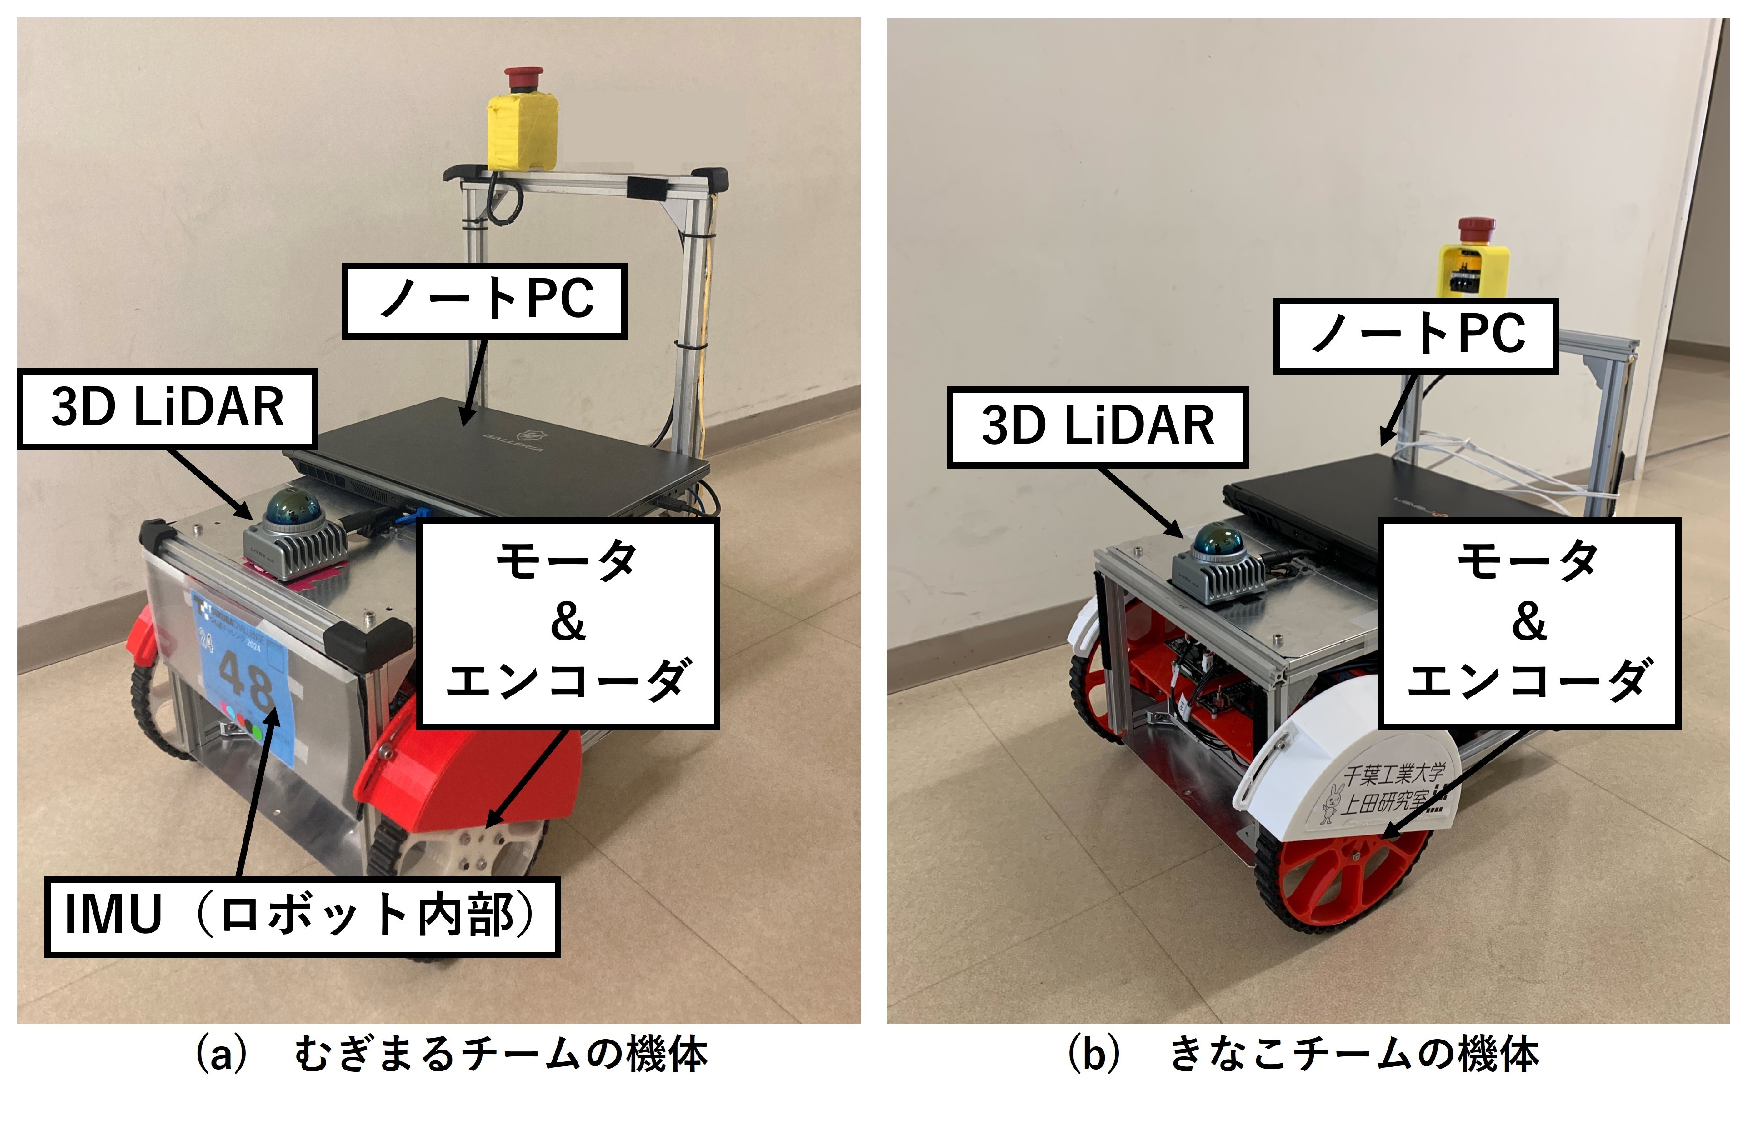
\includegraphics[width=1.0\linewidth]{figs/robot.eps}
     \caption{各チームの機体}
     \label{fig:robot}
   \end{center}
 \end{figure}

%\begin{figure}[H]
%  \label{fig:robot}
%  \begin{minipage}[b]{0.48\columnwidth}
%    \centering
%    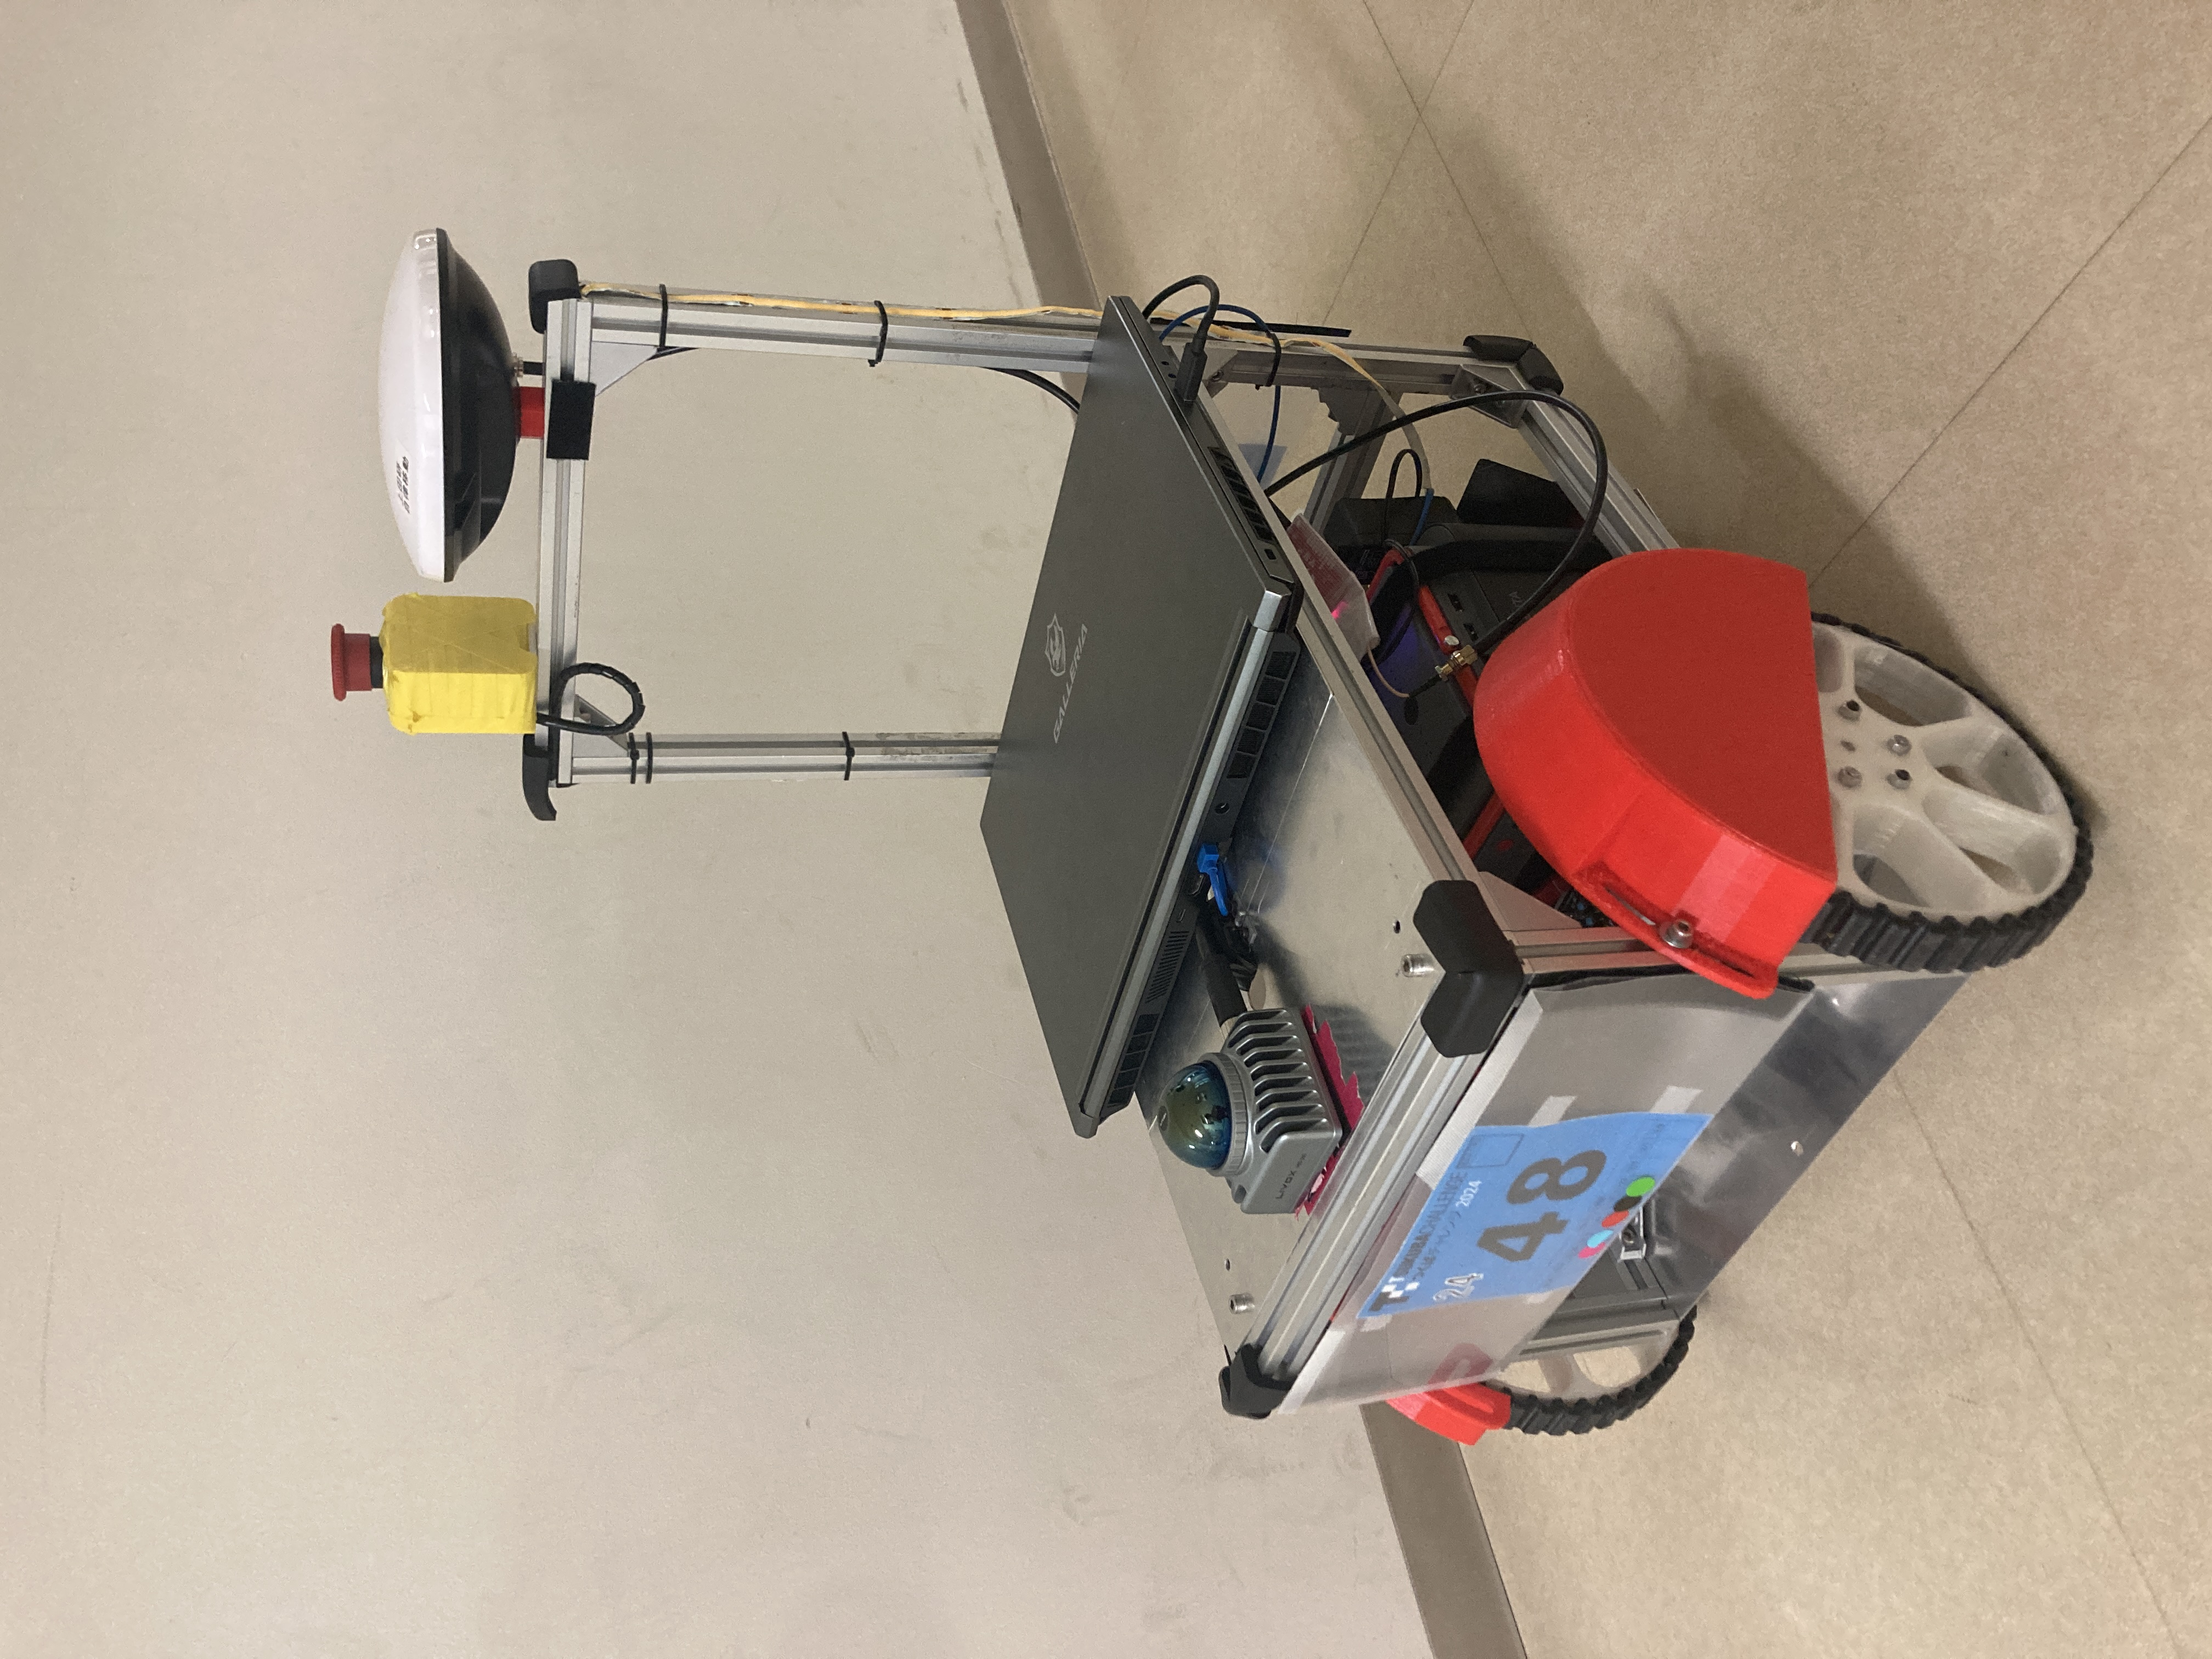
\includegraphics[width=1.0\columnwidth]{figs/mugimaru_robot_2024.eps}
%    %\label{mugimaru_robot}
%  \end{minipage}
%  \begin{minipage}[b]{0.48\columnwidth}
%    \centering
%    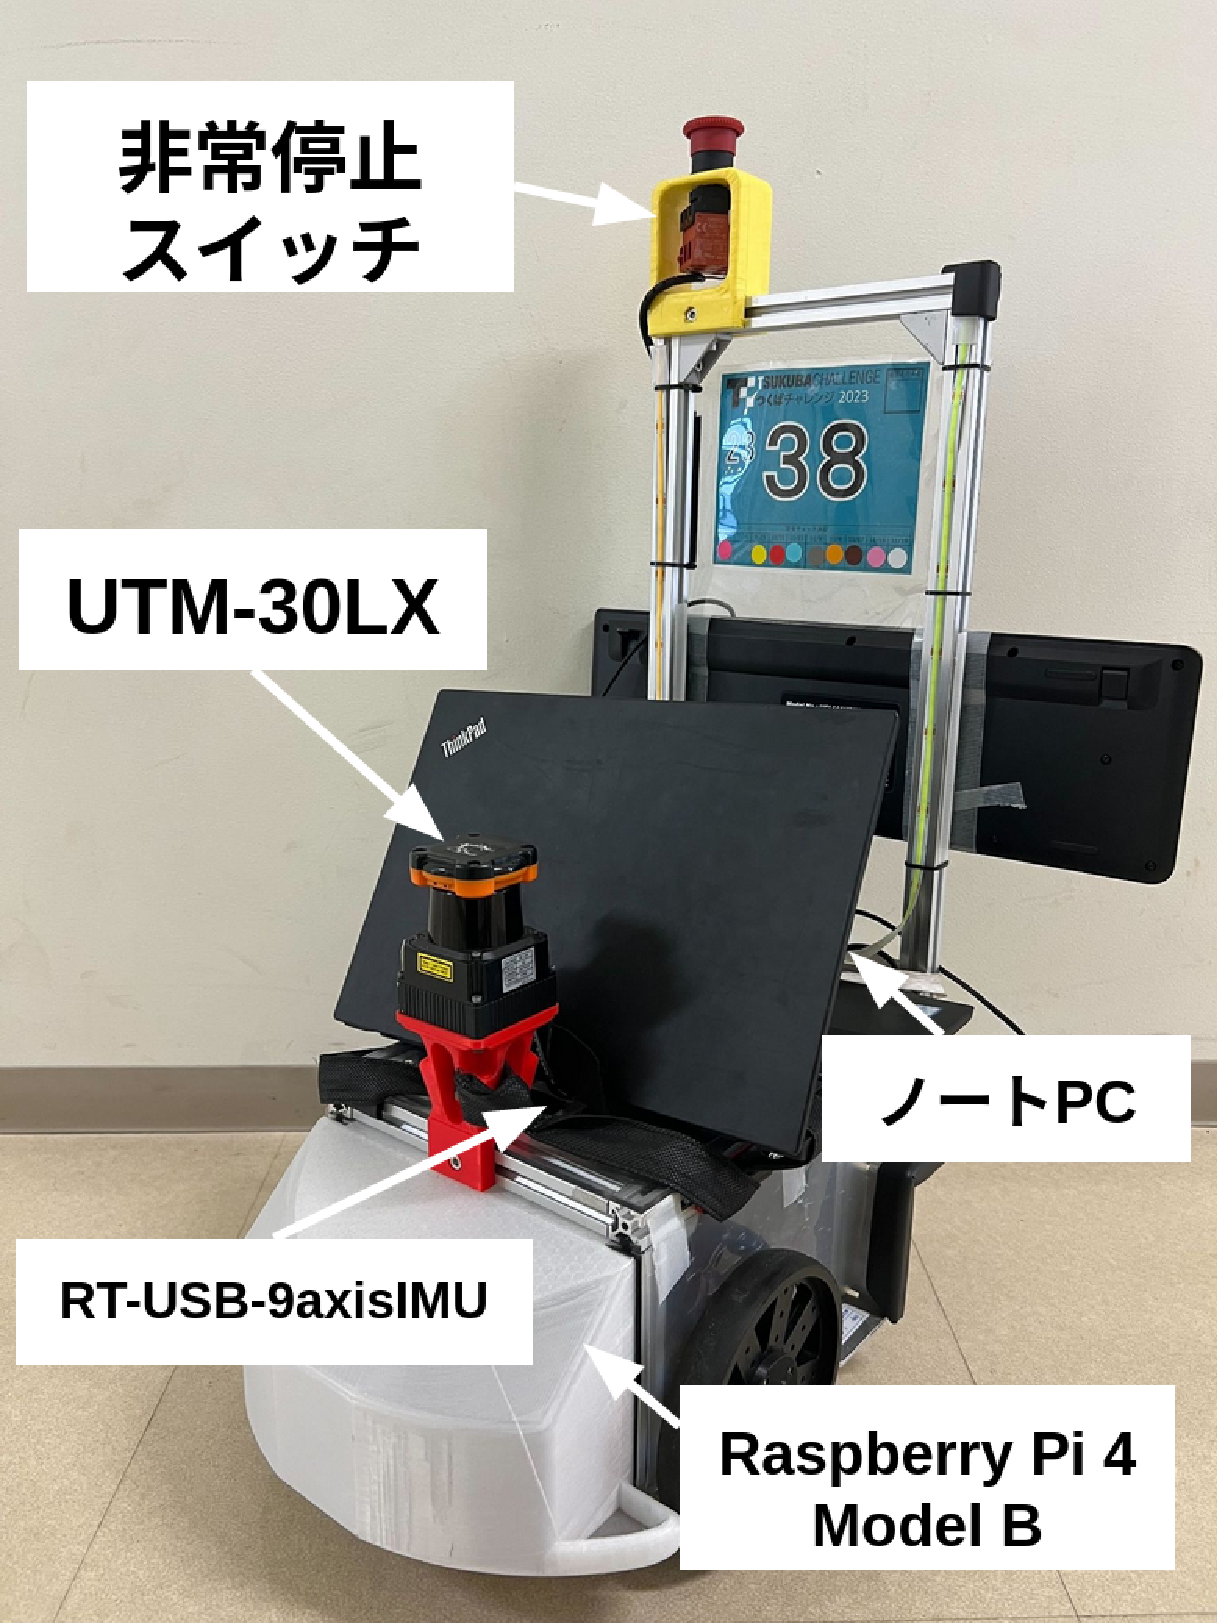
\includegraphics[width=1.0\columnwidth]{figs/tama_robot.pdf}
%    %\label{kinako_robot}
%  \end{minipage}
%  \caption{左: むぎまるチームの機体 右: きなこチームの機体}
%\end{figure}


計算機は, 各チームのロボットとも
ノートPCとRaspberry Piの2台を搭載している. 
Raspberry Piでモータの制御など低レイヤーの処理を行い, 
上位レベルの処理はノートPCが担う. 
ノートPCの諸元を表\ref{table:laptop}に示す. 

\begin{table}[H]
  \centering
  \caption{各チームのノートPCの諸元}
  \label{table:laptop}
  % \begin{tabular}{|l|p{4.0cm}|p{1.0cm}|}
	  \begin{tabular}{|l|p{5.0cm}|l|}
    \hline
    チーム   & CPU & RAM\\ 
    \hline
    むぎまる & AMD Ryzen 5 5600h with radeon graphics & 16GB \\ 
		  %@@@↑こっちは®とかつけないの?
    \hline
    きなこ   & 12th Gen Intel® Core™ i7-12700H  & 32GB \\
    \hline
  \end{tabular}
\end{table}

センサ構成としては, 両チームともに,
Raspberry Pi Cat標準のエンコーダと, 
3D LiDAR(Livox Mid-360)を使用している. 
むぎまるチームはさらに, アールティ社の 
IMUセンサモジュール(RT-USB-9axisIMU2\cite{RTshopIMU})を使用している.

ソフトウェアは, 
両チームともROS 2\cite{ROS 2}をベースに構築した. 
ソフトウェアの詳細については, 
次節以降で説明する. 


\subsection{むぎまるチーム}

%\subsubsection{システム構成}
むぎまるチームのシステム構成について説明する。
ロボットに搭載した計算機、センサ、アクチュエータの接続の関係及び
計算機で実行するROS 2ノードの概要を表したものを
図\ref{fig:mugimaru_system}に示す。

Raspberry Piには、IMUとエンコーダ、車輪駆動用の
モータを接続した。
実行するノードとしては、IMU用のROS 2ドライバーノードと、
オドメトリの出力とモータの制御を実施するノードがある。
後者のノードでは、エンコーダの値と
前者のノードで配信されたIMUの情報からロボットのオドメトリを計算し、
トピックとして配信する。
モータの制御は、外部のノードからトピックとして受信した
ロボットの速度指令をもとに実行する。

PCには、3D LiDARとRaspberry Piを接続した。
実行するノードとしては、3D LiDAR用のノードが2つ、
ロボットの自己位置推定とナビゲーションを実行するノードがある。
3D LiDAR用のノードとしては、Livox用のROS 2ドライバーノードと、
3D LiDARからの3次元点群を2次元に圧縮し、
トピックとして配信するノードがある。
自己位置推定には、emcl2\_ros2パッケージ\cite{emcl2_ros2}を使用した。
このパッケージでは、走行する環境の地図と
オドメトリ、2次元のLiDARデータを使用して、
ロボットの推定位置をtfの形式で出力する。
地図の作成には、slam\_toolboxパッケージ\cite{slam_toolbox}を使用した。
ナビゲーションには、navigation2パッケージ\cite{nav2}を使用した。



\begin{figure}[h]
  \begin{center}
    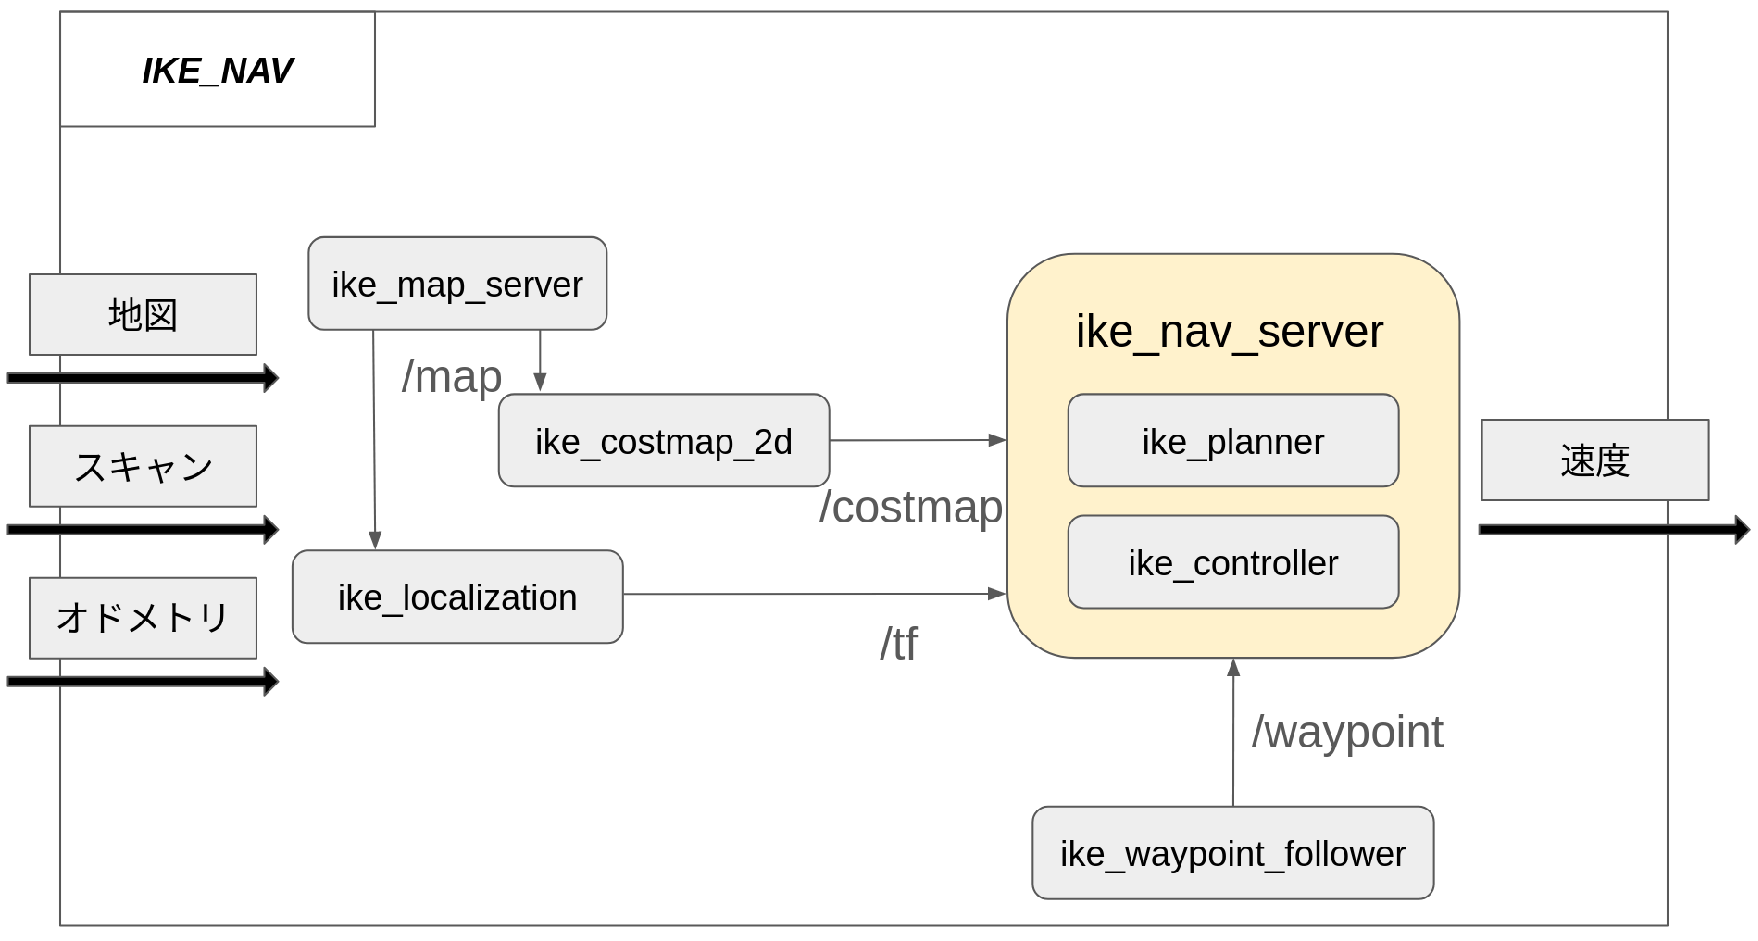
\includegraphics[width=1.0\linewidth]{figs/ike_nav.pdf}
    \caption{むぎまるチームのシステム構成}
    \label{fig:mugimaru_system}
  \end{center}
\end{figure}



\subsection{きなこチーム}\label{sub:localization}

\subsubsection{概要}

きなこチームでも, むぎまるチーム同様, 
自己位置推定にemcl2\_ros2, ナビゲーションにnavigation2を採用したが, 
チームの目標である自己位置推定の信頼性向上のため, 
emcl2\_ros2に手を入れた. 
具体的には, 3D LiDARの3次元点群を高さ別に分け, 
それぞれの高さで2次元の地図を作り, 
走行中に利用する2次元地図を切り替えるというものである. 
これにより, たとえば人が多いところでは地上から離れた
高さの地図を使ったり, 場所ごとに
より特徴に富んだ高さの地図を使い分けたりすることができる. 
また, 地図と同じ高さのスキャンデータを使用することで, 
マップとスキャンデータの特徴の対応関係をより正確にさせている. 
3次元の自己位置推定を用いないのは, 
計算量の削減を指向したからである. 
%@@@↑あってます?

%開発の背景には, 人や車などの動的障害物による自己位置推定の破綻という課題があった. 
%当初この問題に対し, 動的障害物の影響を受けにくい2m以上の高さの点群データのみを使用する手法を採用していた. 
%自己位置推定手法はむぎまるチームと同じように, 3次元マップとセンサから得られる点群データは, 高さ方向(z軸)の情報を圧縮し2次元平面(xy平面)に投影し, 2次元マップと2次元のスキャンデータによる自己位置推定を実現していた. 
%しかし, 環境の特徴は場所によって異なる高さに存在する. 
%そのため, この手法では重要な特徴が失われ, 自己位置推定が不安定になる問題が発生していた. 
%この課題を解決するため, ロボットの現在位置に応じて自己位置推定に使用するマップとスキャンデータの高さ範囲を動的に変更するシステムを新たに開発した. 


\subsubsection{システム構成}
システムの開発のために以下の2つのパッケージを作成した. 

\begin{itemize}
  \item map\_manager: 複数の2次元マップと高さ範囲のパラメータを管理
    \begin{itemize}
      \item ロボットが指定した領域に進入すると, その領域に最適化された2次元マップと高さパラメータを提供
    \end{itemize}
  \item pointcloud\_to\_dual\_scan: 3D LiDARのスキャンデータから2種類の2次元スキャンデータを生成
        \begin{itemize}
          \item 障害物回避用のスキャンデータ
          \item 自己位置推定用のスキャンデータ(map\_managerの指定する高さ範囲に基づく)
        \end{itemize}
\end{itemize}
%@@@ここは絶対に空行をあけないこと!
map\_managerは, 事前に作成した複数の2次元占有格子地図を保持している. 
これらの地図は, 3D LiDARとIMUを統合したSLAM技術であるGLIM\cite{glim}を用いて作成した3次元マップから, 必要な高さ領域を抽出して変換したものである. 

\subsubsection{システム統合}
図\ref{fig:kinako_system}に示すように, 3D LiDARから取得したスキャンデータはpointcloud\_to\_dual\_scanで処理され, 2種類の2次元スキャンデータに変換される. 
map\_managerは, ロボットの位置に応じて最適な2次元マップと高さパラメータを提供し, 自己位置推定を安定させる. 
navigation2により生成された速度指令値はraspimouseを介してモータードライバに伝達され, ロボットの制御を実現している. 

\begin{figure}[h]
  \begin{center}
    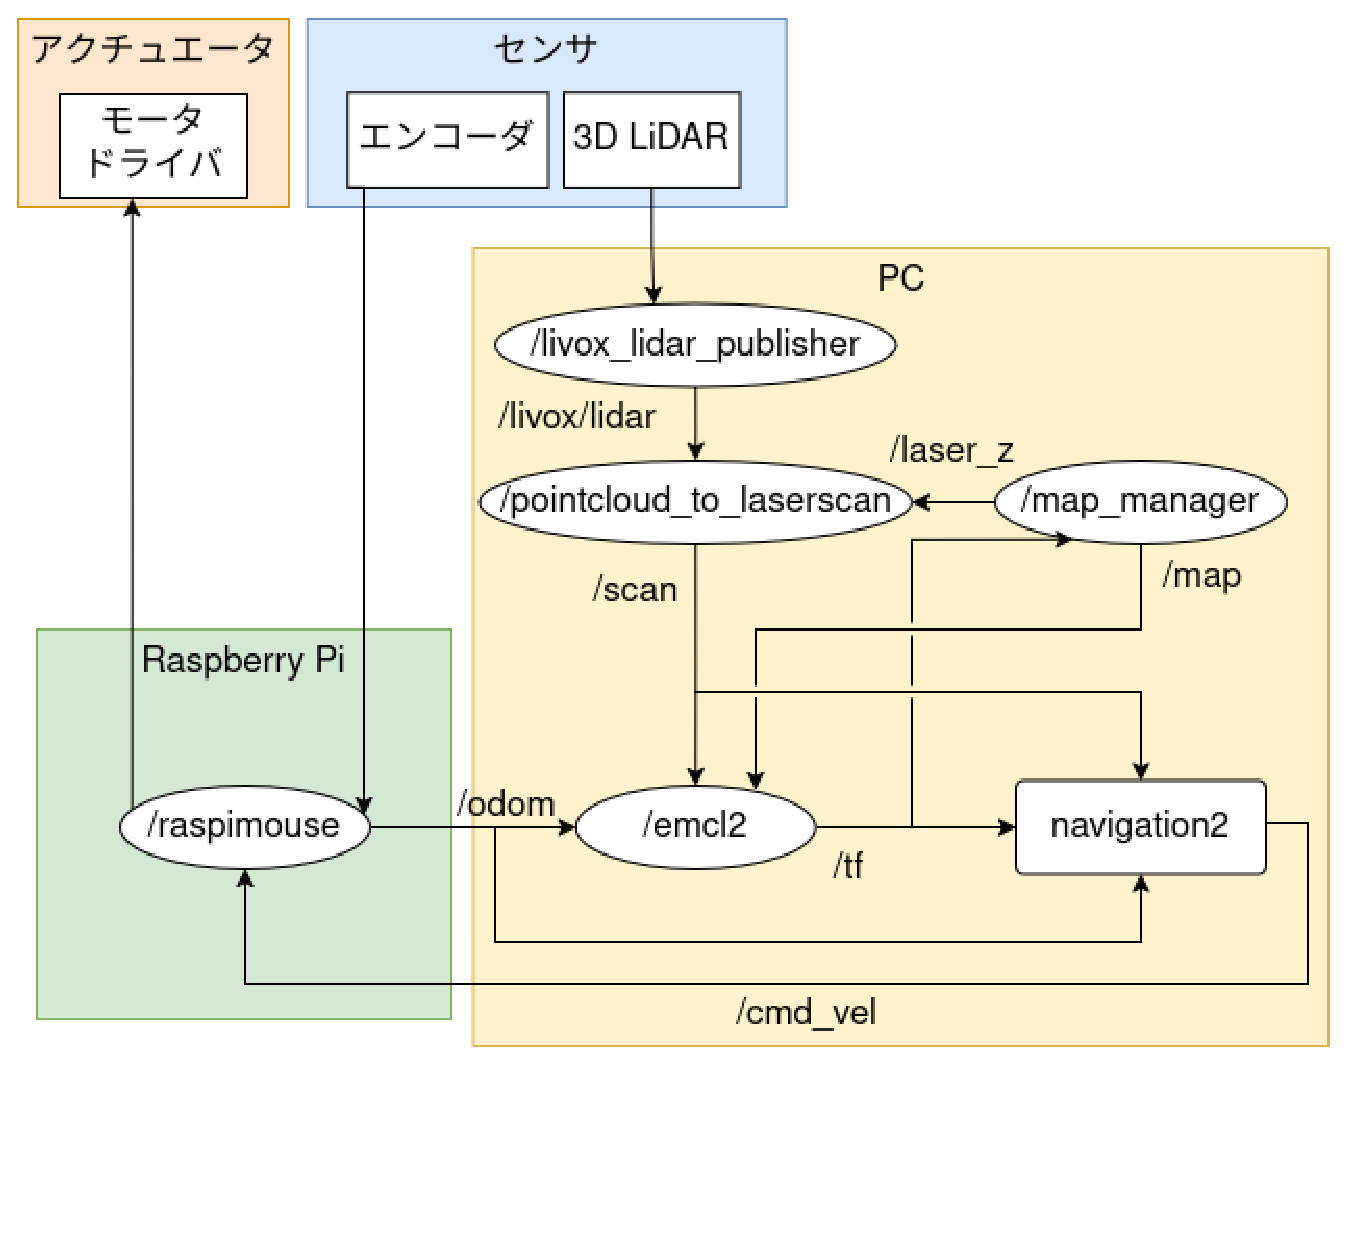
\includegraphics[width=1.0\linewidth]{figs/kinako_system_2024.eps}
    \caption{きなこチームのシステム構成}
    \label{fig:kinako_system}
  \end{center}
\end{figure}


\section{本走行の結果}

つくばチャレンジ2024での本走行の結果を表\ref{MainRun}に示す. 
%@@@ちゃんと総括する文を入れましょう. 

\begin{table}[H]
  \caption{各チームの本走行の結果}
  \label{MainRun}
  \begin{tabular}{|c|c|p{4.0cm}|}
    \hline
    チーム         & 走行距離 & リタイアの理由\\
    \hline
    むぎまるチーム & 470 m    & 横断歩道の途中でロボットが長時間動けなくなりその場でリタイア\\
    \hline

    きなこチーム  & 6m    & スタート直後に左へ旋回し,道路へコースアウトしたためリタイア \\
    \hline
  \end{tabular}
\end{table}

\subsection{むぎまるチーム}
\subsubsection{本走行・実験走行で見つかった課題}
\paragraph{走行不可能領域への侵入でロボットが動作不能になる問題}
むぎまるチームは本走行において, 横断歩道の途中で
navigation2がナビゲーションを中断し, 
動作不能に陥ったことでリタイアとなった. 
この原因は, navigation2が経路生成時に参照するコストマップにおいて, 
ロボットが走行できない領域(以降「走行不可能領域」)に侵入したことであった. 
%↑@@@文分けましょう. あるいは図を見せる前から細かすぎるのでもっと要約する. 
この状況をRVizを用いて可視化した際の画像を図\ref{fig:mugimaru_result}に示す. 
図中のピンク色の範囲は走行不可能領域のコスト, 
水色の範囲はロボットの内接円半径を考慮した走行不可能領域のコストを表している. 
つまり, ロボットの中心が水色の範囲に侵入すると
ロボットが走行不可能領域にいると判断される. 
%%%中心の話をするなら画像内でも中心を表現したほうが見やすい気がする. 
%%%↑図に中心の表現を追加
図\ref{fig:mugimaru_result}からロボットの中心は
水色の範囲に侵入していることが確認できる. 
この状態になった後, プランナーから
%@@@これは使うプランナーによる@@@
経路及び動作の生成が実施されなかった. 
その後, リカバリー動作が実行されたが, 
有効に働かずナビゲーションを中断してしまった. 

この問題への対策としては, 
グローバルプランナーで経路を算出する方法ではなく, 
文献\cite{ueda2023JRM}で用いられている価値反復のように, 
ロボットが存在しうる位置, 向きすべてに対して行動を
割り付ける方法(最適方策を求める方法)を導入することが考えられる. 
価値反復の場合は, 走行に適さない位置に
(無限大ではない)大きなペナルティーを与えておき, 
その領域で行動計画をすると, 
そこから脱出する行動が割り付けられるので, 
動作が中断されることはない. 


%この問題への対策として, 走行可能領域に入るまで
%障害物を回避しながら動き回るという復帰動作を実装することが
%一つ挙げられる. 
%図からロボットの前方には走行可能領域があることが確認できる. 
%その場所までLiDARにより周囲の障害物を検知して, 
%それらを回避しながら移動可能であれば, 
%この問題が発生した場合にでもナビゲーションを続行できるようになると考える. 


\begin{figure}[h]
  \begin{center}
  	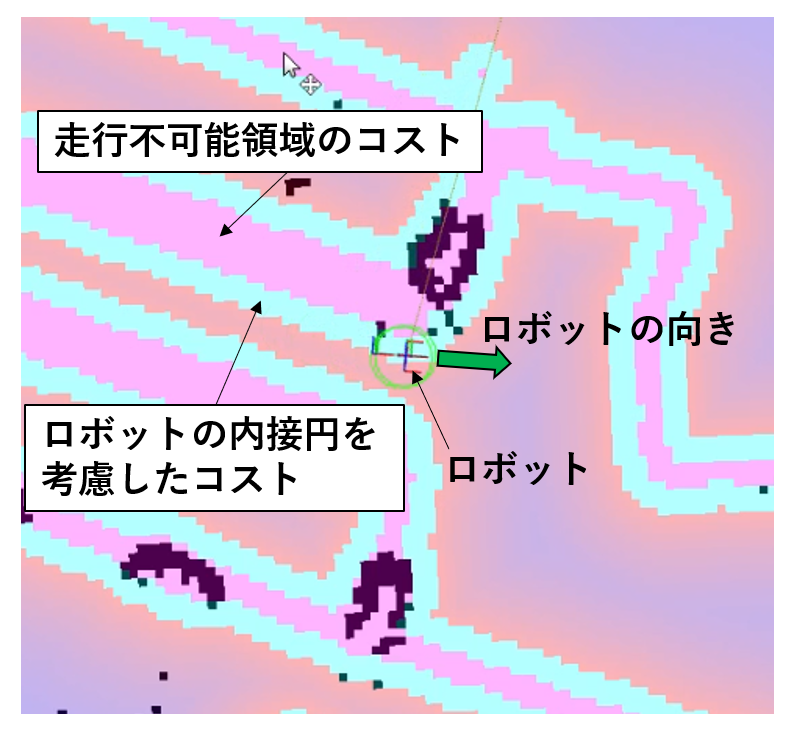
\includegraphics[width=0.9\linewidth]{figs/mugimaru_result.eps}
  	\caption{ロボットが走行不可能領域に侵入したときの図} 
  	\label{fig:mugimaru_result}
  \end{center}
\end{figure}



\subsection{きなこチーム}
\subsubsection{本走行の結果}
きなこチームは本走行開始直後, グローバル経路に沿って進まず想定外の左旋回を行い道路に出たため, 走行距離6mで終了となった. 
このときのログを確認したところ, 正常なナビゲーションが行われていないことが分かった. 
%%%正常なナビゲーションが行われていなかったデータがほしい
%%% or 〜〜があった。そのため、正常なナビゲーションが行われていなかったと考えられる。
大会当日, グローバル経路生成後に緊急停止スイッチを押し2分ほど待機すると, navigation2の更新周期が維持できなくなり, 処理遅延やタイムアウトが頻発するという問題が発生した. 
通常, このような問題はCPUやメモリの過負荷状態で観察される現象である. 
この問題は大会当日は再現性を持って発生したものの, 後日の検証では再現することができなかった. 
今後, 根本的な原因を特定するために, さらなるの調査を行っていく予定である. 

\subsubsection{実験走行で発生した問題}
実験走行中に以下の技術的な問題が発生した. 

1. 狭い通路で起きた問題\\
実験走行時, 狭い通路でロボットが回転し止まらなくなることが何度かあった. 
navigation2のログを解析した結果, 以下の処理が行われていたことが確認できた. 

\begin{enumerate}
  \item 障害物との距離が近いためロボットの周囲ローカルコストマップが飽和
  \item ローカルプランナーのパスを生成できずリカバリの動作として回転を開始
  \item  一定時間回転後に速度指令値を0にする処理を実行
\end{enumerate}

しかし, 3の処理が実行されていたにも関わらず、実際のロボットは静止せず回転を続けていた. 
実際の挙動とシステムの指令値の不一致について, 原因を究明するための調査を行っていく予定である. 

2. 動的障害物への対応の遅れ\\
動的障害物に対するグローバル経路の更新が遅く, オペレーターが緊急停止を押さなければ衝突してしまう場面があった. 
また, システムが動的障害物の進行方向に経路を設定することがあり, 円滑な走行の妨げとなった. 
これに対する対策として、グローバルプランナーの更新周期の最適化と動的な障害物の移動方向を考慮したグローバル経路の生成のアルゴリズム改良が挙げられる。


\section{その他の試み}

つくばチャレンジの環境において試していない
研究室での取り組みについて紹介する. 
紹介したものついては, 来年度以降のつくばチャレンジで
試すことを考えている. 

当研究室では, 価値反復アルゴリズムを
移動ロボットの経路計画へ適用した
パッケージを開発している\cite{ueda2023JRM}. 
価値反復アルゴリズムは,
最適制御問題を解くことができるアルゴリズムである. \cite{上田詳解}
このアルゴリズムで現在地から目的地までの経路を求める大域計画
を行うことで, 最適な経路(最短時間で移動できる経路)を算出することができる. 
また, この計算結果を障害物回避を行う局所計画にも流用することで, 
大域計画と局所計画が競合することなく, 
障害物を環境全域を用いて迂回をする経路も算出することができる. 
一方で, 価値反復アルゴリズムには, A*など移動ロボットの経路計画に
一般によく用いられるアルゴリズムと比べ, 
計算量が多く計算にかかる時間が長いという欠点がある. 
しかし, 近年の計算機の性能の向上によって
実時間で経路計画を行うことが可能となっている. 

また, 価値反復パッケージに関連する研究も行っている. 
価値反復アルゴリズムとA*を組み合わせて走り出しまでの
時間を短縮する研究\cite{中村2024}
では, 価値反復アルゴリズムの計算量が多いために
目的地に向かって走り出すまで時間がかかる問題の解決に取り組んでいる. 


%文献\cite{上田2023}では, 
%自己位置推定の不確かさを考慮した行動決定
%を実現するために, パーティクルの分布から直接行動を決定する
%手法を実装している. 
%この手法を実用できると,自己位置推定の結果が不確かであれば,
%センシングできない縁石などの障害物から遠ざかって移動するなど,
%よりロボットが安全に走行できるようになる. 

%計算機の能力があがっていくことを見越して, 
%A*探索などより計算量の大きい価値反復を利用した, 
%ナビゲーションパッケージを開発している. 
%このパッケージでは, 
%地図中の任意の場所からゴールまでに移動する経路を
%完全に解くことにより, 歩行者などの地図に載っていない
%障害物(移動障害物)を発見したときに最適な迂回路をすばやく
%計算することを実現している. 



%文献\cite{ikebeMECH}では, 
%人混みなどにおける自己位置推定の破綻を防ぐための研究を行っている. 
%これはつくばチャレンジのスタート地点に人が多く集まることに
%注目して行っている研究である. 
%研究している手法は, 
%MCLの各パーティクルに「視野」を持たせ, 
%移動障害物を見ているパーティクルを淘汰することで, 
%移動障害物に起因する誤った情報をMCLに
%取り込まないようにするというものである. 
%この方法は, 各パーティクルの重みを更新するときに
%取り込むセンサ情報が減るので, 
%計算量が減少するという効果がある. 
%この手法の性能調査はシミュレータ上のみで完結しているため, 
%つくばチャレンジ本走行で使用して効果について調査したいと考えている. 


\section{結言}
%%%簡素な構成のロボットで走行したことも書く?
今年度は昨年に引き続きROS 2ベースの
システム構成でつくばチャレンジに参加した. 
それに加え新たな取り組みとして, 
メンテナンス性と搭載量の向上のためにロボットを拡張した. 
ソフトウェア開発の面では, 自己位置推定の破綻に対処可能なパッケージの開発や
動的障害物が多い中でも動作する自己位置推定器の開発に取り組んだ. 
来年度は今年度の開発内容をもとに, 見つかった課題への対策や, 
4章で述べた価値反復を適用した経路計画に取り組み, 
コースの完走を目指す. 


\section*{謝辞}
つくばチャレンジ実行委員会, つくば市の皆様に感謝申し上げます. 
上田研究室の鷲尾優作氏, 三浦璃音氏, 
林原研究室の皆様には, つくばチャレンジ2024の参加にあたりご意見, ご協力頂き感謝申し上げます. 

% 参考文献
% \small
\footnotesize
\begin{thebibliography}{99}

  \bibitem{RTshop}
  株式会社アールティ: ``Raspberry Pi Cat 屋外でも動かせる中型2輪ロボット'',
  RT Robot Shop Products,\url{https://rt-net.jp/products/raspberry-pi-cat/} (last visit 2025-01-29)
  
  \bibitem{RTshopIMU}
  株式会社アールティ: ``USB出力9軸IMUセンサモジュール'',
  RT Robot Shop Products,\url{https://rt-net.jp/products/usb9imu/} (last visit 2025-01-29)

  \bibitem{ROS 2}
  Macenski, Steven {\it et al.}: ``Robot Operating System 2: Design, architecture, and uses in the wild,''
  Science Robotics, Vol. 7, No. 66, 2022.

  \bibitem{ueda2004iros}
  Ryuichi Ueda {\it et al.}: 
  ``Expansion Resetting for Recovery from Fatal Error in Monte Carlo Localization -- Comparison with Sensor Resetting Methods,'' Proc.of IROS,pp.2481--2486,2004.
  
  \bibitem{fox1999etal}
  D. Fox {\it et al.}: ``Monte Carlo Localization: Efficient Position Estimation for Mobile Robots,''
  Proc. of AAAI, pp. 343-349, 1999.
  
  \bibitem{emcl2_ros2}
  Ryuichi Ueda: ``CIT-Autonomous-Robot-Lab/emcl2\_ros2,'' \url{https://github.com/CIT-Autonomous-Robot-Lab/emcl2_ros2} (last visit: 2025-01-22).
  
  \bibitem{slam_toolbox}
  SteveMacenski: ``SteveMacenski/slam\_toolbox,'' \url{https://github.com/SteveMacenski/slam_toolbox} (last visit: 2025-1-27).

  \bibitem{nav2}
  ROS Planning: ``ros-planning/navigation2 (humble branch),'' \url{https://github.com/https://github.com/ros-planning/navigation2.git} (last visit: 2025-1-22).

  \bibitem{上田詳解}
    上田隆一: ``詳解確率ロボティクス'', 講談社, 2019

  \bibitem{上田確率}
    上田隆一: ``ロボットの確率・統計'', コロナ社, 2024

  \bibitem{ueda2023JRM}
  R. Ueda, L. Tonouchi, T. Ikebe, and Y. Hayashibara: ``Implementation of Brute-Force Value Iteration for Mobile Robot Path Planning and Obstacle Bypassing,''
  J. Robot. Mechatron., Vol.35, No.6, pp. 1489-1502, 2023.

   \bibitem{中村2024}
    中村啓太郎,登内リオン,永木悠,林原靖男,上田隆一: ``自律移動ロボットのための価値反復ベースの大域計画器におけるA*探索による暫定経路の算出'',第25回システムインテグレーション部門講演会(SI2024),1F1-11,2024
  %\bibitem{emcl2}
  %Ryuichi Ueda: ``ryuichiueda/emcl2,'' \url{https://github.com/ryuichiueda/emcl2} (last visit: 2024-01-01).

  %\bibitem{池邉2022}
  %池邉 龍宏,内田 璃空,畑中 優一郎,臼井 温希,庄司 史門,松井 大和,山崎 政光,登内 リオン,林原 靖男,上田 隆一: Raspberry Pi のみを計算に用いる小型移動ロボットでのつくばチャレンジ 2022 参加レポート,つくばチャレンジ2022シンポジウム予稿集,2022.

  %\bibitem{ROS}
  %Morgan Quigley {\it et al.}: ``ROS: an open-source Robot Operating System,''
  %Open-Source Software workshop of the International Conference on Robotics and Automation, 2009.

  %\bibitem{fox2003}
  %Dieter Fox:
  %``Adapting the Sample Size in Particle Filters Through KLD-Sampling,''
  %International Journal of Robotics Research, Vol. 22, No. 12, pp. 985-1003, 2003.

  %\bibitem{gutmann2002}
  %Jens-Steffen Gutmann and Dieter Fox:
  %``An Experimental Comparison of Localization Methods Continued,''
  %Proc. of the IEEE/RSJ International Conference on Intelligent Robots and Systems (IROS),pp. 454-459, 2002.

  % \bibitem{ueda2002tdp}
  % 	Ryuichi Ueda {\it et al.}: 
  % ``Team description of Team ARAIBO,'' 
  % Proc. of 2002 International RoboCup Symposium, 2002. 

  % \bibitem{map2gazebo}
  % Shiloh Curtis: ``shilohc/map2gazebo'',\url{https://github.com/shilohc/map2gazebo} (last visit: 2021-12-31).

  % \bibitem{move_base}
  % Eitan Marder-Eppstein: ``move\_base,'' \url{http://wiki.ros.org/move_base} (last visit: 2021-12-31).

  %\bibitem{amcl}
  %Brian Gerkey: ``amcl,'' \url{https://wiki.ros.org/amcl} (last visit: 2021-12-31).

  %\bibitem{gmapping}
  %Brian Gerkey: ``gmapping,'' \url{http://wiki.ros.org/gmapping} (last visit: 2021-12-31).

  % \bibitem{GIMP}
  % GIMP.org: ``GIMP,'' \url{https://www.gimp.org/} (last visit: 2021-12-31).



  %\bibitem{raspicat}
  %Ryuichi Ueda and Daisuke Sato: ``ja/raspicat,'' \url{https://wiki.ros.org/ja/raspicat} (last visit: 2021-12-31).

  %\bibitem{youtube}
  %BEIKE: ``つくばチャレンジ2022 実験走行 11/19 スタートからゴールまで自律移動(神の手4回),'' \url{https://www.youtube.com/watch?v=3gpjVhRIJDY} (last visit: 2022-12-12).

  % \bibitem{raspicat_rosbag}
  % Tatsuhiro Ikebe: ``uhobeike/raspicat\_rosbag,'' \url{https://github.com/uhobeike/raspicat_rosbag} (last visit: 2021-12-31).

  %\bibitem{池邉2021}
  %池邉 龍宏,曹 越,高橋 秀太,クルス ペレス アントニオ,林原 靖男,上田 隆一: 小型移動ロボットによるつくばチャレンジへの挑戦,第22回計測自動制御学会システムインテグレーション部門講演会,pp.3390-3393,2021.

  

  % \bibitem{上田2019}
  % 上田 隆一: ``詳解確率ロボティクス'', 講談社, 2019.

  %   \bibitem{上田2020}
  %  上田隆一,鈴木勇矢: 自己位置が不確かな状況における移動ロボットの危険回避行動の生成,第38回日本ロボット学会学術講演会予稿集,pp.RSJ2020AC2C2-02,オンライン開催,2020.

  % \bibitem{地図合成}
  % 川合隆太他: ``産業技術大学院大学における自律移動ロボット「産技大2号」の開発'',2019年度つくばチャレンジシンポジウム, pp.4-7, 2020.


  % \bibitem{aws2020}
  %   CIT自律ロボット研究室: ``AWSロボットデリバリーチャレンジで本研究室メンバーが優勝,'' \url{https://lab.ueda.tech/?post=20200915_aws_challenge} (last visit 2022-01-04)

  % \bibitem{学科サイト}
  %   千葉工業大学先進工学部未来ロボティクス学科: ``AWS Robot Delivery Challenge 2021 準優勝'', \url{https://www.robotics.it-chiba.ac.jp/j/?p=838} (last visit 2022-01-04)

  % \bibitem{つくばチャレンジロボット仕様}
  % つくばチャレンジ実行委員会事務局:``つくばチャレンジ 2021 ロボット仕様条件'',
  % \url{https://tsukubachallenge.jp/2021/regulations/specs} (last visit 2021-12-31)

  % \bibitem{UST-30LX}
  % 北陽電機株式会社: ``UST-30LX'',\url{https://www.hokuyo-aut.co.jp/search/single.php?serial=195#spec} (last visit: 2021-12-31).

  % \bibitem{Turtlebot3 Burger}
  % 株式会社ロボティズ: ``Turtlebot3 Burgerの仕様'',\url{https://emanual.robotis.com/docs/en/platform/turtlebot3/features/} (last visit: 2022-1-3).

  % \bibitem{つくばチャレンジ公式記録}
  % つくばチャレンジ実行委員会事務局:``つくばチャレンジ2021の走行結果'',
  % \url{https://tsukubachallenge.jp/2021/records/final} (last visit 2021-12-31)

  % \bibitem{出野畑中}
  %   畑中 優一郎,出野 廣太郎,上田 隆一:``Raspberry Pi 3BのみでRaspberry Pi Catのナビゲーション(屋内環境編)'',CIT自律ロボット研究室,\url{https://lab.ueda.tech/?post=20211210} (last visit 2022-01-02)

  %\bibitem{ike_nav}
  %Tatsuhiro Ikebe: ``uhobeike/ike\_nav,'' \url{https://github.com/uhobeike/ike_nav} (last visit: 2024-01-10).

  %\bibitem{ike_nav_detail}
  %池邉龍宏: ``自作ナビゲーションスタックでつくばチャレンジ2023に挑戦してみた話'',
  %\url{https://qiita.com/BEIKE/items/f3ff141cc25d49c01363} (last visit 2023-1-10).



  %\bibitem{hart1968}
  %Peter E. Hart and Nils J. Nilsson and Bertram Raphael: ``A Formal Basis for the Heuristic Determination of Minimal Cost Paths,''
  %IEEE Transactions on Systems Science and Cybernetics, Vol. 4, No.2, pp. 100-107, 1968.

  %\bibitem{dijkstra1959}
  %E. W. Dijkstra : ``A Note on Two Problems in Connexion with Graphs,''
  %Numerische Mathematik, Vol. 1, pp. 269-271, 1959.

  %\bibitem{alberto2006}
  %Bemporad, Alberto: ``Model Predictive Control Design: New Trends and Tools,''
  %Proceedings of the 45th IEEE Conference on Decision and Control, pp. 6678-6683, 2006.

  %\bibitem{fastlio}
  %Ericsii: ``Ericsii/FAST\_LIO (ros2 branch),'' \url{https://github.com/Ericsii/FAST_LIO.git} (last visit: 2023-11-19).

  %\bibitem{autoware}
  %The Autoware Foundation: ``autowarefoundation/autoware.universe,'' \url{https://github.com/autowarefoundation/autoware.universe.git} (last visit: 2023-11-19).


  %\bibitem{ike_nav_loc_youtube}
  %池邉龍宏: ``自作パッケージで屋外自律移動してみた in つくばチャレンジ2023(本走行)'',
  %\url{https://www.youtube.com/embed/k9yxRKOCa14?si=c7ISmE1wH5W4BhgU&amp;start=1365} (last visit 2024-01-05)

%\bibitem{上田2023}
%上田隆一, 登内リオン, 池邉龍宏, 林原靖男: ``移動ロボットのための自己位置の不確かさを考慮したセンシングできない固定障害物の回避手法 ---価値反復を用いたナビゲーションにおける状態空間の局所拡張---'', 第28回ロボティクスシンポジア講演論文集, pp. 118-123, 2023.

  %\bibitem{tonouchi2023}
  %登内リオン, 池邉龍宏, 林原靖男, 上田隆一: ``価値反復を用いた移動ロボットによる屋外ナビゲーション,''
  %日本機械学会ロボティクス・メカトロニクス講演会, 2P1-G06, 2023.


  %\bibitem{ikebeMECH}
  %池邉龍宏, 林原靖男, 上田隆一: ``未知障害物によるモンテカルロ自己位置推定の破綻を防ぐための観測範囲の制限と選択'',
  %日本機械学会ロボティクス・メカトロニクス講演会, 2A2-G06, 2023.


\end{thebibliography}
\normalsize

\clearpage

%\section{付録として, 各実験走行でどんなことをやっていたかを書く?}
% 当チームは, 9日間分のすべての実験走行会に参加した. 
% 7月2日, 7月23日は確認走行区間から信号あり横断歩道手前までの自己位置推定のテストを行った. 
% 地図は昨年作ったものを使い, 自己位置推定のパッケージにemcl2を使った. 
% また, 駅・公園エリアの地図作成のためのrosbagを取った. 
% 9月17日, 10月1日は駅・公園エリアの走行実験を行った. 
% 走行エリアが増えたことに伴い地図の容量が増大し, 4GBメモリのRaspberry Piでは処理できなかった. 
% メモリの容量を増やし, 地図の余白部分を削ることで駅・公園エリアが走行できるようになった. 
% 10月22日, 10月23日は信号あり横断歩道の横断の走行テストを行った. 
% 通常の走行速度では青信号中に横断しきれなかったため, 
% 信号あり横断歩道の横断中のみ走行速度を変えることで, 青信号中に横断しきることができた. 

\end{document}
